\documentclass[11pt]{report}

\usepackage[utf8]{inputenc}
\usepackage{graphicx,caption,setspace}
\usepackage{subcaption}
\usepackage{geometry}   \geometry{margin=1.25in}
\usepackage{amsmath}
\usepackage{xcolor}
\usepackage{float}
\usepackage{longtable}
\usepackage{multirow}
\usepackage{amssymb}
\usepackage{pifont}
\usepackage{rotating}
\usepackage{pdfpages}

\usepackage{natbib}
\usepackage[nonumberlist]{glossaries}
\makeglossaries
\loadglsentries{glossary}

\captionsetup{font={stretch=1.1}}
% \renewcommand{\baselinestretch}{1.2}
\setstretch{1.25}

\usepackage{fancyhdr}
\pagestyle{fancy}
\fancyhead{}
\setlength{\headheight}{14pt}
\fancyhead[R]{Guitar Effects Auditioning System}
\fancyfoot{}
\fancyfoot[C]{\thepage}
\fancyfoot[R]{Chapter \thechapter: \Chaptername}
\fancyfoot[L]{Nicholas Pham}

\newcommand{\insertimage}[4] {
	\begin{figure}[!htbp]
		\centering
		\captionsetup{width= #1 \textwidth}
		\includegraphics[width = #1\textwidth]{#2}
		\caption{#3}
		\label{#4}
	\end{figure}
}

\let\Sectionmark\sectionmark
\def\sectionmark#1{\def\Sectionname{#1}\Sectionmark{#1}}
\let\Chaptermark\chaptermark
\def\chaptermark#1{\def\Chaptername{#1}\Chaptermark{#1}}

\newcommand{\sect}[1] {
	\section*{#1}
	\addcontentsline{toc}{section}{#1}
	\stepcounter{section}
	\sectionmark{#1}
}
\newcommand{\chpt}[1] {
	\chapter*{#1}
	\addcontentsline{toc}{chapter}{#1}
	\stepcounter{chapter}
	\chaptermark{#1}
}


\fancypagestyle{appendix}{
	\fancyhead{}
	\setlength{\headheight}{14pt}
	\fancyhead[R]{Guitar Effects Auditioning System}
	\fancyfoot{}
	\fancyfoot[C]{\thepage}
	\fancyfoot[R]{\Sectionname}
	\fancyfoot[L]{Nicholas Pham}
}

\newcommand{\cmark}{\ding{51}}	% check mark
\newcommand{\xmark}{\ding{55}}	% x mark

\newcommand{\kohm}{k$\Omega$\:}
\newcommand{\Mohm}{M$\Omega$\:}
\newcommand{\ohm}{$\Omega$\:}

\newcommand{\uF}{$\mu$F\:}

\begin{document}

	\pagestyle{plain}
	\begin{titlepage}
	\begin{center}
		\vspace*{0.5in}
		\huge
		\textbf{Hot Swappable Guitar Effects Pedal Auditioning System}\\
		\vspace*{1in}
		\Large
		\textbf{Nicholas Pham} \\
		S.B. Candidate in Electrical Engineering \\
		\vspace*{0.5in}
		\textbf{Advisors: Jim MacAurthur, Scott Kuindersma}

		\vfill

		A senior design project submitted in partial fulfillment of the reqirements for the degree of Bachelor of Science at Harvard University. \\
		\vspace*{0.1in}

		
\includegraphics[width = 0.1\textwidth]{FinalImages/Harvard_shield-University.png}\\
		
		\vspace*{0.1in}
	    Harvard University School of Engineering and Applied Science \\
	    Cambridge, Massachusetts \\
	    April 5, 2019
	\end{center}
\end{titlepage}

	\thispagestyle{plain}
\begin{center}
    \Large
    \textbf{Hot Swappable Guitar Effects Pedal Auditioning System}
    
    \vspace{0.4cm}
    \large
    \textbf{Nicholas Pham}
    
    \vspace{0.9cm}
    \textbf{Abstract}
\end{center}
Lorem ipsum dolor sit amet, consectetur adipisicing elit, sed do eiusmod tempor incididunt ut labore et dolore magna aliqua. Ut enim ad minim veniam, quis nostrud exercitation ullamco laboris nisi ut aliquip ex ea commodo consequat. Duis aute irure dolor in reprehenderit in voluptate velit esse cillum dolore eu fugiat nulla pariatur. Excepteur sint occaecat cupidatat non proident, sunt in culpa qui officia deserunt mollit anim id est laborum.

	\tableofcontents

	\listoffigures

	\listoftables

	\pagestyle{fancy}

	\chapter{Introduction}	% combine the intro and problem definition into one chapter
	what are guitar effects pedals?

\section{Current Auditioning Methods}
Lorem ipsum dolor sit amet, consectetur adipisicing elit, sed do eiusmod tempor incididunt ut labore et dolore magna aliqua. Ut enim ad minim veniam, quis nostrud exercitation ullamco laboris nisi ut aliquip ex ea commodo consequat. Duis aute irure dolor in reprehenderit in voluptate velit esse cillum dolore eu fugiat nulla pariatur. Excepteur sint occaecat cupidatat non proident, sunt in culpa qui officia deserunt mollit anim id est laborum.
Lorem ipsum dolor sit amet, consectetur adipisicing elit, sed do eiusmod tempor incididunt ut labore et dolore magna aliqua. Ut enim ad minim veniam, quis nostrud exercitation ullamco laboris nisi ut aliquip ex ea commodo consequat. Duis aute irure dolor in reprehenderit in voluptate velit esse cillum dolore eu fugiat nulla pariatur. Excepteur sint occaecat cupidatat non proident, sunt in culpa qui officia deserunt mollit anim id est laborum.
Lorem ipsum dolor sit amet, consectetur adipisicing elit, sed do eiusmod tempor incididunt ut labore et dolore magna aliqua. Ut enim ad minim veniam, quis nostrud exercitation ullamco laboris nisi ut aliquip ex ea commodo consequat. Duis aute irure dolor in reprehenderit in voluptate velit esse cillum dolore eu fugiat nulla pariatur. Excepteur sint occaecat cupidatat non proident, sunt in culpa qui officia deserunt mollit anim id est laborum.
Lorem ipsum dolor sit amet, consectetur adipisicing elit, sed do eiusmod tempor incididunt ut labore et dolore magna aliqua. Ut enim ad minim veniam, quis nostrud exercitation ullamco laboris nisi ut aliquip ex ea commodo consequat. Duis aute irure dolor in reprehenderit in voluptate velit esse cillum dolore eu fugiat nulla pariatur. Excepteur sint occaecat cupidatat non proident, sunt in culpa qui officia deserunt mollit anim id est laborum.
Lorem ipsum dolor sit amet, consectetur adipisicing elit, sed do eiusmod tempor incididunt ut labore et dolore magna aliqua. Ut enim ad minim veniam, quis nostrud exercitation ullamco laboris nisi ut aliquip ex ea commodo consequat. Duis aute irure dolor in reprehenderit in voluptate velit esse cillum dolore eu fugiat nulla pariatur. Excepteur sint occaecat cupidatat non proident, sunt in culpa qui officia deserunt mollit anim id est laborum.
Lorem ipsum dolor sit amet, consectetur adipisicing elit, sed do eiusmod tempor incididunt ut labore et dolore magna aliqua. Ut enim ad minim veniam, quis nostrud exercitation ullamco laboris nisi ut aliquip ex ea commodo consequat. Duis aute irure dolor in reprehenderit in voluptate velit esse cillum dolore eu fugiat nulla pariatur. Excepteur sint occaecat cupidatat non proident, sunt in culpa qui officia deserunt mollit anim id est laborum.
Lorem ipsum dolor sit amet, consectetur adipisicing elit, sed do eiusmod tempor incididunt ut labore et dolore magna aliqua. Ut enim ad minim veniam, quis nostrud exercitation ullamco laboris nisi ut aliquip ex ea commodo consequat. Duis aute irure dolor in reprehenderit in voluptate velit esse cillum dolore eu fugiat nulla pariatur. Excepteur sint occaecat cupidatat non proident, sunt in culpa qui officia deserunt mollit anim id est laborum.
Lorem ipsum dolor sit amet, consectetur adipisicing elit, sed do eiusmod tempor incididunt ut labore et dolore magna aliqua. Ut enim ad minim veniam, quis nostrud exercitation ullamco laboris nisi ut aliquip ex ea commodo consequat. Duis aute irure dolor in reprehenderit in voluptate velit esse cillum dolore eu fugiat nulla pariatur. Excepteur sint occaecat cupidatat non proident, sunt in culpa qui officia deserunt mollit anim id est laborum.
Lorem ipsum dolor sit amet, consectetur adipisicing elit, sed do eiusmod tempor incididunt ut labore et dolore magna aliqua. Ut enim ad minim veniam, quis nostrud exercitation ullamco laboris nisi ut aliquip ex ea commodo consequat. Duis aute irure dolor in reprehenderit in voluptate velit esse cillum dolore eu fugiat nulla pariatur. Excepteur sint occaecat cupidatat non proident, sunt in culpa qui officia deserunt mollit anim id est laborum.

\subsection{Permenant Display Board}

\subsection{Free Connection Method}
	\section{Problem Statement}

The benefits and drawbacks of the two guitar effects pedal auditioning methods are summarized in Table \ref{tab:prev_method_pro_con}.  Clearly, neither method is ideal, and the issues resulting from each's drawbacks are a detriment to both potential customers and to retailers.  Therefore, guitarists need an improved process to audition guitar pedals to facilitate more expedient and accurate purchasing decisions.

	\begin{table}
	\begin{center}
	\renewcommand{\arraystretch}{2}
	\captionsetup{justification=centering}
	\caption{Summary of Current Guitar Effects Pedal Auditioning Methods.  \\A good solution system would combine the benefits of both methods.}
	\raggedbottom
	\begin{tabular}{|c|c p{2in}|c p{2in}|}
		\hline
		\multirow{2}{*}{Method} & \multicolumn{4}{c|}{Attributes} \\
		 & \multicolumn{2}{c}{Ease of Use} & \multicolumn{2}{c|}{Flexibility} \\
		\hline
		Display Board & 
		\cmark & 
		Just activate footswitch to engage effects &
		\xmark &
		Single manufacturer; fixed routing order; potential signal degradation unavoidable\\

		\hline

		Free Connection &
		\xmark & 
		Requires plugging and unplugging signal and power; generally slow
		&
		\cmark & 
		Any manufacturer; many connection topologies possible; power supply can be selected\\
		\hline
	\end{tabular}
	\label{tab:prev_method_pro_con}
	\end{center}
	\end{table}

\section{Design Requirements}

In practice, a solution should combine the best attributes of the two current methods.  This involves fulfilling two broad categories of requirements.  The requirements of the first category ensure that the solution shows a functional improvement over the previous methods; it should solve the problem described in the problem statement.  The most pertinent requirement for this is a reduction in the "swap time", or the time required to switch between two pedals in an A-B test.  This fundamental situation is important to any sort of auditioning.  To make it worth the effort of going through this project and for retail stores to implement, a solution should offer a major improvement in swap time.  An order of magnitude improvement seems like a reach goal, but an 80\% improvement in swap time over the free connection method is reasonable.

In order for the solution to be effective, it must be usable with a majority of pedals available at typical retail locations.  An 80\% market coverage is reasonable because a majority of retailer stock contains pedals by just a handful of brands.  There is a trade-off between universal compatibility versus form and function, so designing for every possible pedal should not be a priority, though a solution design should not preclude an eventual expansion of compatibility.

For a retail store to use a solution, the cost to implement it in the store should not be obtrusive.  As the solution developed in this project is not intended to be production ready, the material cost rather than the final cost is specified.  A initial cost of \$200 should cover the main part of the system, and the incremental cost to make any additional pedals compatible with the system should be no more than \$20 per pedal.  The latter cost is a more important point, because many retail stores may stock hundreds of guitar pedals, so the individual cost must 

Finally, the solution system should be as intuitive as possible.  This is not easy to quantify, though a simple metric might be the number of words required to give useful working knowledge of the system in a user guide.  However, this seems fairly artificial, as an instruction manual could be continually optimized to reduce word count ad nauseam, so performing an actual verification measurement on this requirement would be rather contrived.  Instead, this requirement should be kept in mind during the design phase as an important consideration.

The second set of requirements deals with the ability of the system to be an unbiased method of comparison, adding no coloration to the sound.  These signal quality properties include signal-to-noise ratio (SNR) and frequency response.  The signal-to-noise ratio of the electric guitar itself, by virtue of its simple passive magnetic pickups, can be very high.  Preliminary measurements suggested an SNR around $90dB$.  Higher values in a controlled environment are likely.  Noise in guitar audio is particularly important, as guitar amplifiers apply a high level of compression and amplification which can significantly increase the noise floor at the speaker.  Particular care must be taken to reduce noise earlier in the signal chain to prevent its amplification.  Most guitar effects are specified with SNR ranging from $80-120dB$, but some of these manufacturer-supplied specifications may be over-inflated, and in most cases are A-weighted, deemphasizing certain parts of the frequency spectrum.  Thus, a $90dB$ SNR is a good baseline requirement.

As in any audio system, the solution's frequency response should be flat across the audio range.  Because very subtle differences in the timbre and frequency content resulting from the use of different pedals is vitally important, a $0.1dBu$\footnote{Note that $dBu$ is a standard audio unit compared to a reference voltage resulting from a $600\Omega$ load dissipating $1mW$ of power.  $0dBu = 0.775V_{rms}$.} flatness is required across the audio frequency range $20Hz$ - $20kHz$.  Performance down to very low frequencies or even DC would be useful for some subharmonic effects and synthesizer pedals, so this would be a plus.

In addition to these signal quality considerations that are important during the actual listening process, the system should also have a short switching time so the user perceives no delay when swapping a pedal in or out of the system.  Because it should be easily achievable with most switching method that might be used while being short enough to have no perceived discontinuities, the system should have a switching time of no longer than $20ms$.  Note that this is the time required by the system to switch signals and is a separate requirement than the swapping time described above.

Finally, to ensure the safety of the equipment following the solution system, switching transients should be limited when switching a pedal in or out of the system.  The transients added by the system should be no larger than $0.5dBu$.

These requirements are summarized in Table \ref{tab:requirements}

	\begin{table}
	\begin{center}
	\captionsetup{justification=centering}
	\caption{Summary of Design Requirements.}
	\renewcommand{\arraystretch}{2}
	\raggedbottom
	\begin{tabular}{|c|c|p{2in}|}
		\hline
		Metric & Target Value & Notes \\
		\hline
		Swap Time 			& 80\% Reduction 	&	\\
		Compatibility 		& 80\%	 		 	&	\\
		System cost 		& \$200				& Materials cost for the initial system	\\
		Incremental cost 	& \$20 				& Materials cost for each additional pedal that is made compatible with the system. \\
		SNR 				& $90dBu$ 			& 	\\
		Frequency Response  & $0.1dBu$ flat over $20Hz - 20kHz$ 	& \\
		Switching Time 		& $20ms$ 			& \\
		Transient 			& $0.5dBu$ 			& Transient added by system during switching \\
		\hline
	\end{tabular}
	\label{tab:requirements}
	\end{center}
	\end{table}

	\chapter{System Design}
	\section{System Overview}

\section{Design Details}
	\subsection{Universal Adaptor}
		\subsubsection{Pedal-Plate Mounting}
		\subsubsection{Plate Size}
		\subsubsection{Plate Material}
	\subsection{Hot Swapping Device}
		\subsubsection{Electrical Connection Mechanism}
		\subsubsection{Pedal Power Selection}
		\subsubsection{Hot Swap Event Detection}
		\subsubsection{Hot Swap Event Actuation}
	\subsection{Analog Signal Routing}
		\subsubsection{Routing Architecture}
		\subsubsection{Analog Voltage Supply}
	\subsection{User Interface}


	\chapter{System Implementation}
	\section{Circuit Board Layouts}
	\subsection{Circuit Board Hierarchy}
	\subsection{Component Placement Considerations}
	\subsection{Routing Considerations}
\section{Circuit Board Assembly}
\section{Mechanical Assembly}

	\chapter{System Evaluation}
	\section{Functional Improvements}

The first main category of system evaluation measurements are related to determining if this solution was successful in solving the problem: did it actually allow guitarists to more easily and quickly test out guitar effects pedals?  

	\subsection{Swap Time}
		\subsubsection{Experiment Description}
		The most important measurement related to this is comparing the time required for users to swap between pedals.  This experiment used to measure this difference was designed to simulate the expected operating conditions of the system.  In this case, each participant conducted four tasks, and the time required to complete each of these tasks was recorded.  For each task, the user began wearing a guitar with its output connected through a single guitar pedal.  They were instructed to safely remove this guitar pedal from the signal chain, and set it down in a defined location.  Then they were instructed to touch a second location before re-inserted the pedal back into the signal chain.


		\insertimage{0.8}{PR5Images/SwapTimeSetup.png}{Swap Time Experimental Setup.  Top: Starting and Ending position, with guitar pedal fully connected.  Bottom: Unplugged position, with guitar pedal disconnected and placed in the blue box in the upper left.  In this experiment, the subjects started in the fully connected position, moved to the unplugged position, touched the blue rectangle on left with one hand and then returned to the fully connected position.  This imitates the process of swapping between two guitar pedals.}{fig:swaptime_setup}


		\begin{table}
		\begin{center}
		\begin{tabular}{ |c|p{8cm}| }
		\hline
		Type Name & Description \\ 
		\hline
		$A$ & Standard sized pedal with side mounted jacks (similar to a Boss Compact pedal) \\
		$B$ & Standard sized pedal with top mounted jacks (similar to the EarthQuaker Devices Bit Commander) \\
		$C$ & Wide pedal with side mounted jacks (similar to Electro Harmonix B9) \\
		\hline
		\end{tabular}
		\caption{Set of three pedals used to represent the range of available products in the swap time test.}
		\label{tab:swaptest_pedals} 
		\end{center}
		\end{table}


		The first three tasks were controls, each conducted with a different standard guitar effects pedal.  These test pedals were chosen to represent some of the breadth of products available on the market (see Table \ref{tab:swaptest_pedals} for details).  The guitar pedal was connected in the standard way, with an instrument cable connected from the output of the guitar to the input of the pedal.  The output of the pedal was connected to the input of a guitar amplifier.  The pedal was powered with a standard $9VDC$ wall wart adapter.  To begin, the participant started with their hands on the guitar.  The pedal was set on a table of standard height to mimic the environment of testing pedals in a guitar store, instead of on the floor.  After a countdown to let the participant know when to start, the timer was started.  From here, the participant disconnected the pedal, placed it in a rectangle marked on the table (shown in Figure \ref{fig:swaptime_setup} as the blue rectangle on the right), then proceeded to touch the second marker (the blue square on the left of the same image).  This simulated the need for a user to grab a second pedal without the experiment actually requiring the use of two separate but identical pedals for each task.  After touching this marker, the participant returned to the larger blue rectangle to grab the pedal and re-insert it into the signal chain, making the required input, output, and power connections.  At this point, once, the participant placed their hands back on the guitar as if to continue playing to test the sound of this "new" pedal, the timer was stopped and the time recorded.  This measurement represents the time required to swap between pedals in the standard manual method.

		The second test tests the hypothesis that the solution decreased the swapping time.  This time the device was sitting on the table, with the instrument cable from the guitar plugged into its master input, and its master output connected to the input of a guitar amplifier.  One of the pedals used for the control was connected to a plate (only one needed to be used for these tests because the mechanics of the swap event is the same regardless of which pedal is being used).  Before the task began, this pedal and plate are inserted into one of the hot-swap connector receiving units.  Again, the participant began with their hands on the guitar and followed the same sequence of steps as before, but this time instead of needing to unplug all of the cables, they needed only remove the plate from the receiver before placing it in the blue rectangle.  During the second half of the task, they again needed only insert the plate into the receiver rather than plugging in cables.

		\subsubsection{Results}
		Six participants were used for this experiment, and each participant performed three trials of each task.  Figure \ref{fig:swaptime_data} shows the averages and standard deviations for each device tested, by participant.  Visually, the plot indicates that there was a clear improvement in the hot swapping solution over all of the other pedals.  It also appears that there were larger variations in the recorded times for the pedals than for the hot swapping solution.  This might be because of the simplicity of the hot swapping solution.  There is little place for error in inserting a plate into the hot swapping receiver, while when plugging in a pedal participants sometimes misaligned the plugs and jacks or even dropped the cable off the table, which is a realistic occurrence.

		\insertimage{0.8}{FinalImages/SwapTime_data.png}{Swap time test data.  Each participant performed the swapping test with three different standard effects pedals (shown in orange, yellow, and purple) as well as with the solution detailed in this report (shown in blue).  The participants performed each test three times, and the average time is shown per participant with standard deviation bars included.}{fig:swaptime_data}

		\subsubsection{Analysis}
		In order to determine if the measurements show success or failure of the solution to meet the design requirements, this data must be synthesized into a single value.  First, the measured times must be converted to a percent time savings by dividing the difference in time between using the hot swapping solution and a standard plugging method by the latter time as a reference:

		$$ r = \% \text{ Reduction} = \frac{t_\text{standard} - t_\text{solution}}{t_\text{standard}} $$

		These data sets are paired by participant, so the percent reduction in time must be calculated for each participant and for each standard pedal tested compared to the participant's time for the hot swapping solution.

		Combining these values requires some sort of averaging, but taking a simple average would not be ideal, as each set of measurements has a different associated standard deviation.  To minimize the variance in the final value, inverse variance weighting was used in taking this average, whereby data points with lower standard deviation are weighted stronger than data points with higher standard deviation.  The weight $w$ for a certain data point $k$ with standard deviation $\sigma$ is given by

		$$ w_k = \frac{1}{\sigma^2} \left( \sum_i \frac{1}{\sigma^2} \right)^{-1} $$

		Then each time reduction data point $r_k$ is weighted by its associated weight and summed to get the average reduction $\overline{R}$:

		$$ \overline{R} = \sum_i r_i w_i $$

		Using this inverse variance weighting, the data indicates that the hot swapping solution has a 65\% time improvement ($\sigma = 8.0\%$) over the standard method.  While this fails to meet the design requirement, which called for an 80\% improvement, it indicates that this solution method shows promise.

		The swap time test provided a clue as to a direction for further improvement.  Many participants had a hard time get the plate to mechanically align with the receiver, which increased the measured time for the solution.  Although sliding one edge in place then letting the rest of the plate fall flat into the receiver is an effective method, this was not discovered by most participants on their own, and most attempted to keep the plate parallel to the table as they inserted it.  A mechanical redesign of the receiver body to include features for guiding the plate into the correct position, including curved or slanted walls instead of right angles might help alleviate this issue and allow the hot swapping method to meet or exceed the 80\% goal.

	\subsection{Compatibility}

		Because of the impracticality of physically testing the solution with many products, this compatibility requirement was designed for during the design phase of the project and thus no tests were conducted in this area.

\section{Signal Quality Verifications}

The second main category of system verification measurements are related to maintaining the same signal integrity as if the guitar were connected directly to the amplifier using an instrument cable.  This allows users to make objective and unbiased comparisons between the products being tested.

	\subsection{Signal-to-Noise Ratio}
		\subsubsection{Measurement Description}
		For this test, an Audio Precision System One (AP) measurement device was used to measure the noise floor of the device under test.  The AP and associated software was used to send programmable test signals through the device and measure the resulting response.  To measure the noise floor, the AP was programmed to output a sinusoid test signal and the amplitude was swept from $+10 dBu$ down to $-100 dBu$.  This corresponds to a sweep from a $6.9Vpp$ signal down to $22\mu Vpp$.

		The plots in Figure \ref{fig:NF_AP} show the amplitude of the measured signal (in $dBu$) plotted against this swept test signal.  When the test signal is above the noise floor, its amplitude dominates the output and the plot shows a straight line with a unit slope.  However, when the test signal's amplitude goes below the noise floor, this dominates, and the slope goes to zero, indicating the level of the noise floor at the measured level of this flat part of the plot.

		The first measurement made was a characterization of the AP itself, with its output and input connected with a two foot coaxial cable.  Measuring the AP's own noise floor shows the limits of observation with this device.

		The important data measurements were then conducted.  Two setups were used, as the signal path which passed only through relays was expected to have a different noise characteristic than the signal path which include the buffers and summing amplifier.

		\subsubsection{Results}

		\begin{figure}[!htbp]
			\centering
			\begin{subfigure}{0.6\textwidth}
				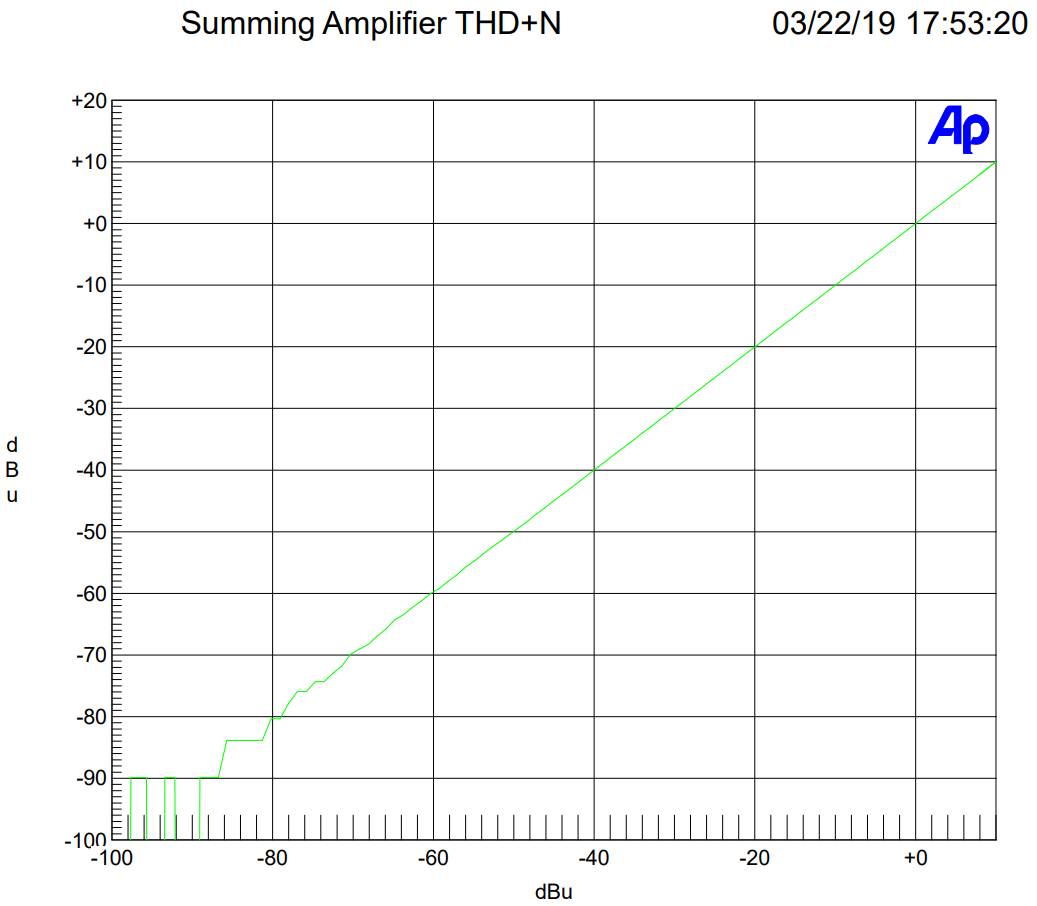
\includegraphics[width = \textwidth]{FinalImages/NF_direct.png}
				\caption{\emph{Direct} routing noise floor measurement output.}
				\label{fig:NF_AP_direct}
			\end{subfigure}
			\vspace{0.5in}
			\begin{subfigure}{0.6\textwidth}
				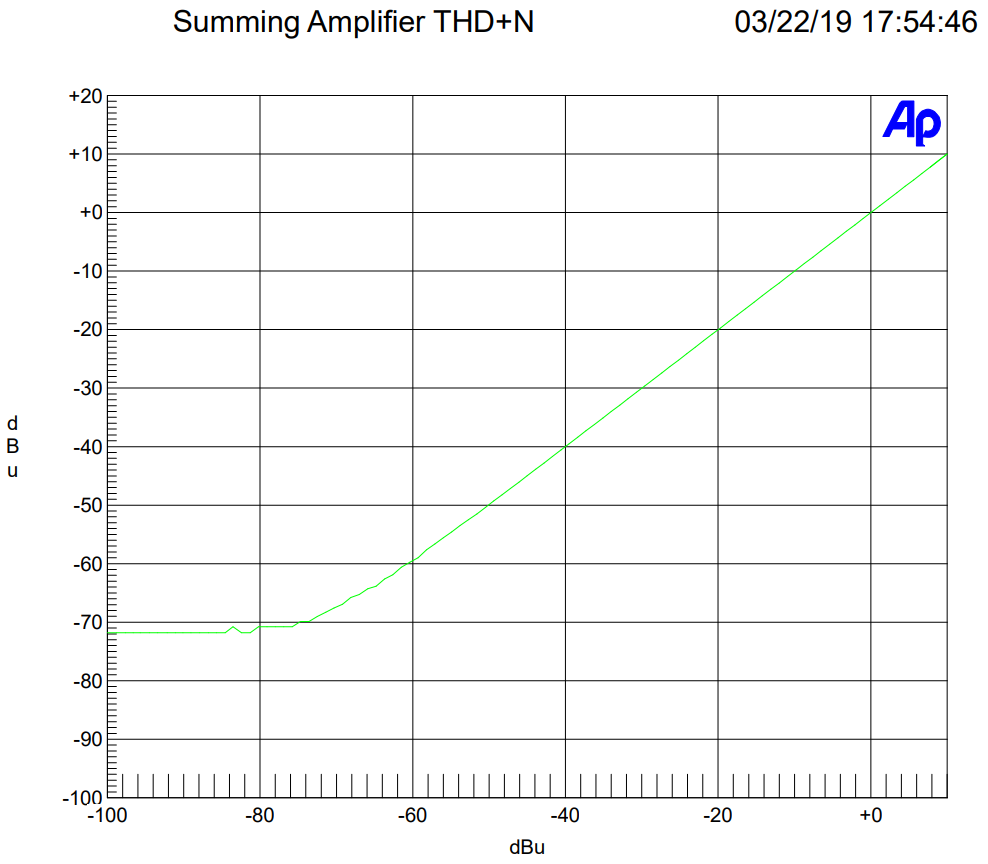
\includegraphics[width = \textwidth]{FinalImages/NF_sum.png}
				\caption{\emph{Summed} routing noise floor measurement output.}
				\label{fig:NF_AP_sum}
			\end{subfigure}
			\caption{Example AP noise floor measurement plots.  The x-axis shows the AP's test sinusoid output amplitude in $dBu$, and the y-axis shows the measured amplitude from the device under test.}
			\label{fig:NF_AP}
		\end{figure}

		During the first measurement, the external switching power supply which had been used was determined to be much more noisy than expected.  During measurements for the prototype in the fall semester, it did exhibit some noise issues, but they were only marginally detrimental to the noise performance.  However, during this test the power supply was demonstrating approximately a $77mV$ noise signal with a strong component near $330Hz$ (equivalent to $-29 dBu$, which resulted in far worse measured noise floor than expected.  The $330Hz$ location of the noise is not something that could be ignored because it is right in the fundamental frequency range of the guitar.  With this in mind, this power supply was replaced with a bench top power supply that did not exhibit any issues.  This lab power supply was used during the rest of the measurements to isolate noise from the device itself.  This is not an unreasonable substitution, as an alternative power supply with a better specification could be easily switched out in the future to solve this issue.

		Both the noise floor measurement from the \emph{direct} signal path which only includes mechanical relays and the measurement from the \emph{summed} signal pat is shown in Figure \ref{fig:SNRbar}.  The bars are referenced to the AP's own noise floor which sets the limit of this measurement.  Lower values indicate better noise performance.  As can be seen, the \emph{direct} signal path performs very well, while the \emph{summed} signal path has a higher noise floor.

		Figure \ref{fig:NF_AP} shows two of the plots generated by the AP software.  Note the strange oscillations in Figure \ref{fig:NF_AP_direct} below $-96dBu$ which suggest that the device's noise floor may be reaching the limits of the measurement system (the plots generated during the characterization of the AP itself showed similar behavior).  On the other hand, Figure \ref{fig:NF_AP_sum} shows more normal behavior of the noise floor overwhelming the test signal.

		\insertimage{0.8}{FinalImages/SNR_bargraph.png}{Results of the noise floor measurements.  The AP's own noise floor was measured to be $-107dBu$.  This was used as a reference value for the other measurements, so effectively the bars show the increase in noise floor over the minimum possible value to be measured; lower values indicate better noise performance.  The \emph{direct} signal path's noise floor was less than $10dBu$ off of the best measurable value, while the summing amplifier performed significantly worse at just $-72.2dBu$.  For all of these measurements, $N=20$ samples were taken.}{fig:SNRbar}


		\subsubsection{Analysis}

		Of course, the noise floor is only one part of the signal to noise ratio; also required is the maximum signal amplitude.  Although in theory the electro mechanical relays can conduct hundreds of volts, this would skew the results of this measurement as guitar pedals would not be expected to output that type of level.  Instead, a reasonable estimation of the maximum signal level would be an $18Vpp$ signal, which would be the largest expected signal from the guitar pedals being tested, as $18V$ is the maximum output of the adjustable regulators supply power to the pedals.  Although some pedals may have internal circuitry to boost their on-board supply voltages above this level, these are few and far between.

		To compute the signal to noise ratio from the measured noise floor and the approximate maximum signal level,

		\begin{align*}
			SNR &= \frac{A_{max}}{A_{noise}} \\
			&= \log(A_{max}) - log(A_{noise})
		\end{align*}

		subtract the noise floor in $dBu$ from the maximum signal level amplitude in $dBu$.  With the two noise floor values recorded in Figure \ref{fig:SNRbar}, the actual signal to noise ratio and can calculated:

		\begin{align*}
			{SNR}_{direct} &= 18.3 - (-96.4) = 114.7 dBu \\
			{SNR}_{summed} &= 18.3 - (-72.2) = 90.5 dBu
		\end{align*}

		Both of these values exceed the design requirement of $90 dBu$, though the \emph{summed} path does not exceed it by much.  These high signal to noise ratios, particular that of the direct, relay-only signal allows users to make informed decisions about the products they audition as they can be sure that this system adds negligible noise.


	\subsection{Frequency Response}
		\subsubsection{Measurement Description}
		The AP system was also used to conduct this test.  Again, the output of the AP was connected to the input of the device under test, and the output of the device under test was connected to the input of the AP.  Here, the AP was programmed to output a sine wave sweep from $50kHz$ down to $10Hz$ at a $0dBu$ amplitude, at 51 discrete frequencies. The AP measured the amplitude of the resulting device output and plotted this against frequency.

		\subsubsection{Results}

		Again, the frequency response was measured for both the \emph{direct} and \emph{summed} signal paths.  Figure \ref{fig:FR_AP} shows the results of the frequency response measurement for both signal paths.  The \emph{direct} signal path measurement in \ref{fig:FR_AP_direct} is very flat down to the minimum frequency.  In fact, the relays should work down to DC.  There is a slight roll off in the upper frequencies mainly above $20kHz$ which could be due to loading from the biasing components used for the summing amplifier and associated buffers.  On the other hand, the \emph{summed} signal path does have a noticeable roll-off in the low frequencies, which appears to start around $100Hz$.  This is a result of the decoupling capacitors used to bias the summing amplifier and buffers to the $A_{Vdd}/2$ virtual ground.

		\begin{figure}[!htbp]
			\centering
			\begin{subfigure}{0.6\textwidth}
				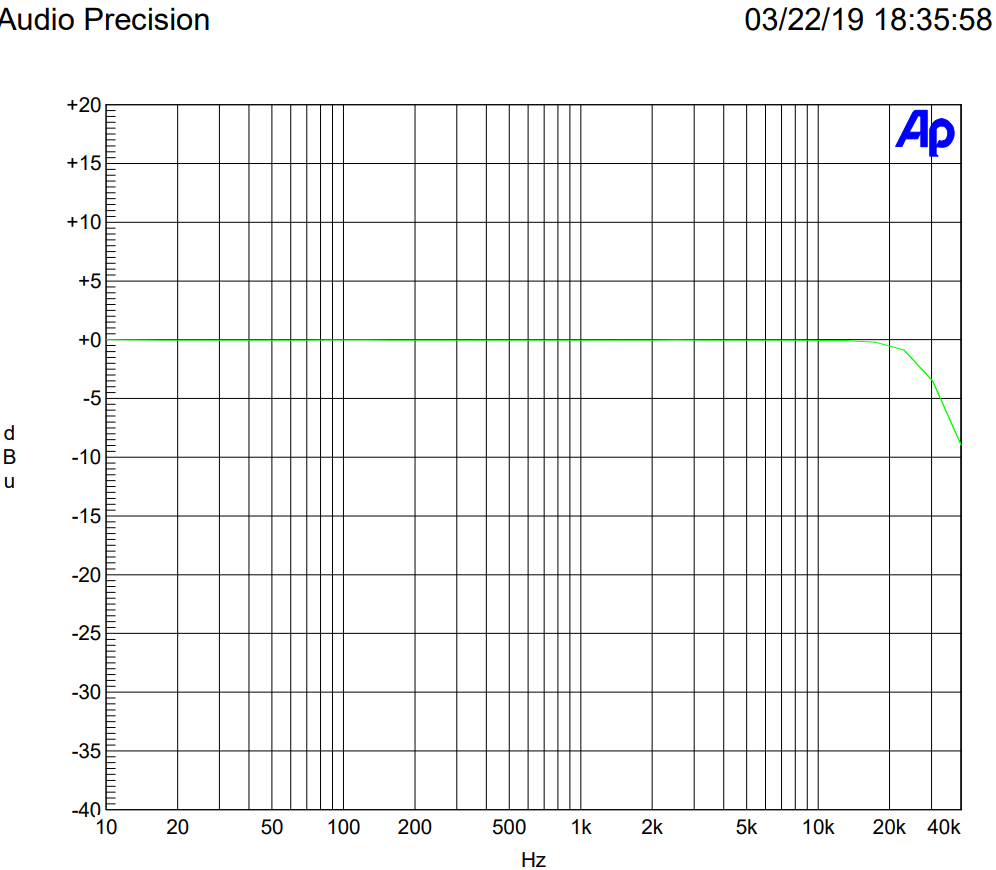
\includegraphics[width = \textwidth]{FinalImages/FR_direct.png}
				\caption{\emph{Direct} routing frequency response measurement output.}
				\label{fig:FR_AP_direct}
			\end{subfigure}
			\begin{subfigure}{0.6\textwidth}
				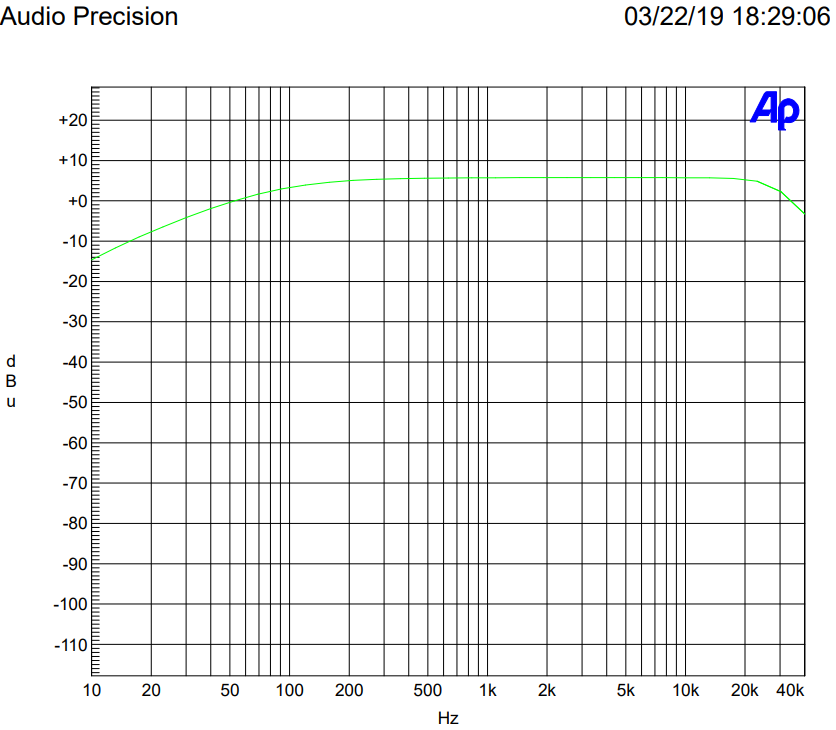
\includegraphics[width = \textwidth]{FinalImages/FR_sum.png}
				\caption{\emph{Summed} routing frequency response measurement output.}
				\label{fig:FR_AP_sum}
			\end{subfigure}
			\caption{Example AP frequency response measurement plots.  The x-axis shows the frequencies of the AP's test sinusoid output amplitude, and the y-axis shows the measured amplitude from the device under test.  Although the high frequency roll off of the \emph{direct} routing appears at first glance to be steeper than that of the \emph{summed} measurement, the scale of the latter plot is longer, so it actuality they have the same slope.  Also note that the flat level of the \emph{summed} test is at $+6dBu$ rather than $0dBu$, which is a result of two $0dBu$ signals being summed.  This means that the latter plot also confirms that the summing amplifier works correctly.}
			\label{fig:FR_AP}
		\end{figure}

		\subsubsection{Analysis}

		To determine if the results of this measurement demonstrate the success or failure of the device to meet the design requirements, the $0.1dBu$ flatness goal was superimposed over the data in the desired frequency range, as seen in .  This was only performed for the \emph{direct} routing configuration, as its accuracy is the most vital.  The rationale for this decision is that when users are using the direct relay-only routing, they are most interested in making subtle comparisons between pedals, so a high performance signal quality specification is paramount.  However, when they use the summing amplifier and splitting features, they are likely more interested in hearing the resulting sound from a combination of pedals, so the signal quality requirements can be slightly relaxed.

		\insertimage{0.8}{PR4Images/FRactive.jpg}{Frequency response of device in active send/receiver mode with signal routing using only relays.  The $0.1dBu$ flatness goal is shown shaded in blue, while the recorded data from the device is plotted as the blue line.  The dashed line at $0dBu$ was the reference signal output by the AP.}{fig:FR_direct}

		As can be seen in Figure \ref{fig:FR_AP_direct}, the device meets this $0.1dBu$ flatness goal.  It makes sense that at no point does the measured signal have a higher amplitude than the reference signal, as the device in this mode is totally passive.  TThe dip in the low frequency is not a big issue, as it occurs around $12Hz$, which is below the audio spectrum, and it still falls within the desired flatness target.

	\subsection{Switching Time}
		\subsubsection{Measurement Description}
		The switching time was measured using the single-shot trigger function of an oscilloscope.  Again the AP was used to output audio signals, in this case sinusoids on both of the channels.  The device output was switched between a direct signal connection to one of the AP outputs and the sum of the two AP outputs.  The trigger level was set higher than the maximum signal level of a single output but below the maximum amplitude of the summed signal.  When the relay switched the output from the single signal to the sum, the oscilloscope triggered and stopped.  The cursors were then used to measure the time difference between when the first signal is lost and begins to float back to ground and when the relay contact stops bouncing and makes solid contact to the second signal.  To capture the relay switching in the opposite direction, one of the AP output signals was inverted so that when the two AP outputs were summed, they canceled, resulting in a lower output.  This was used as the "first" signal, and the trigger level was set to trigger when the relay switched to a single sinusoid.

		\subsubsection{Results}
		Figure \ref{fig:Switchscope} shows one of the oscilloscope traces used to record the switching time measurements.  Twenty trials of each switching direction were performed and their times recorded.

		\insertimage{0.95}{FinalImages/switch2sum.png}{Example oscilloscope trace showing a relay switching event.  This particular capture involved switching from a single signal to a summed signal.  As can be seen at the far left (to the left of cursor $a$), the signal is a sinusoid with an amplitude around $0dBu$.  To the right of cursor $b$ shows the output after the signal switched to the summed signal (now with amplitude $+6dBu$).  In between cursors $a$ and $b$ is the relay switching event.  When the contact blade is disconnected at time $a$, the output floats back to ground for approximately $350\mu s$.  After this, the relay blade begins to connect with the other contact, and the other summed output can begin to be seen.  However it takes a full $\Delta t = b - a = 519 \mu s$ before the bouncing appears to stop.  In this trial, the $519 \mu s$ was recorded as the switching time.}{fig:Switchscope}

		\subsubsection{Analysis}

		Figure \ref{fig:Switchbar} shows the average switching times with the relays switching in both directions.  Though there does appear to be some asymmetry when switching from one output compared to the other, the measurements show that the switching time is much lower than the $20ms$ goal, and will pose no issue with the signal cutting out.

		\insertimage{0.8}{FinalImages/Switch_bargraph.png}{Comparison of average relay switching time in both directions, plotted with standard deviation.  $N = 20$ for both measurements.  Though there appears to be some difference in the switching times between the two directions, the main takeaway from this plot is that the both of these are far less than the $20ms$ requirement.}{fig:Switchbar}

	\subsection{Switching Transient}

	Transients resulting from signal switching can arise from two main sources. The first is the system itself.  This could result from some microphonic components in the system picking up the mechanical vibrations when the relay blade moves between the contacts. It could also result from the relatively large switching current driving the relay or other digital components coupling into the audio signal. If instead a solid state analog switch had been used, the charge injection resulting from stray capacitances in the MOSFET devices could cause a shift in level, resulting a transient when switched.  The oscilloscope images show that the transient size is never greater than the instantaneous difference between the signals being switched, which demonstrates that the relays themselves do not add any transient.

	The other type of transients are related to the signals themselves that are being switched.  Any instantaneous difference in level will result in a transient of some sort.  The worst possible case would be two signals $180^\circ$ out of phase being switched at the moment they have reached their maximum.  This would result in a transient the size of the signals' amplitude.  Because of time constraints and a desire to avoid adding complexity to minimize signal quality issues, no mitigation circuits were designed to reduce this type of transient.  Measuring this type of switching transient is difficult to glean meaningful data from because of this dependence on the exact signals being switched, so no there was no further exploration of this area during this project.

	\chapter{Conclusion}
	\section{Comparing Built Specifications to Design Requirements}
\section{Future Work}

	\newpage

	\begin{center}
	\chapter*{Acknowledgments}
	\addcontentsline{toc}{chapter}{Acknowledgments}

	I would like to thank my thesis reader Scott Kuindersma for suggesting the idea for this project, as well as the ES100 staff for guiding me through this process.  In addition, I could not have made it through this project without the support of my family and friends.  Most importantly, I would like to thank my advisor Jim MacArthur for taking on this project with me and being such a great mentor.  
	\end{center}

	\pagestyle{appendix}

	\chpt{Appendix}

	\sect{Budget}
	The following BOM and other budget materials were generated from the supplied template.  The total cost for the main system was about \$200, which was on track for the requirement.  However, the labor cost for fabrication would be quite high; DFM would be required for real world implementation.  
	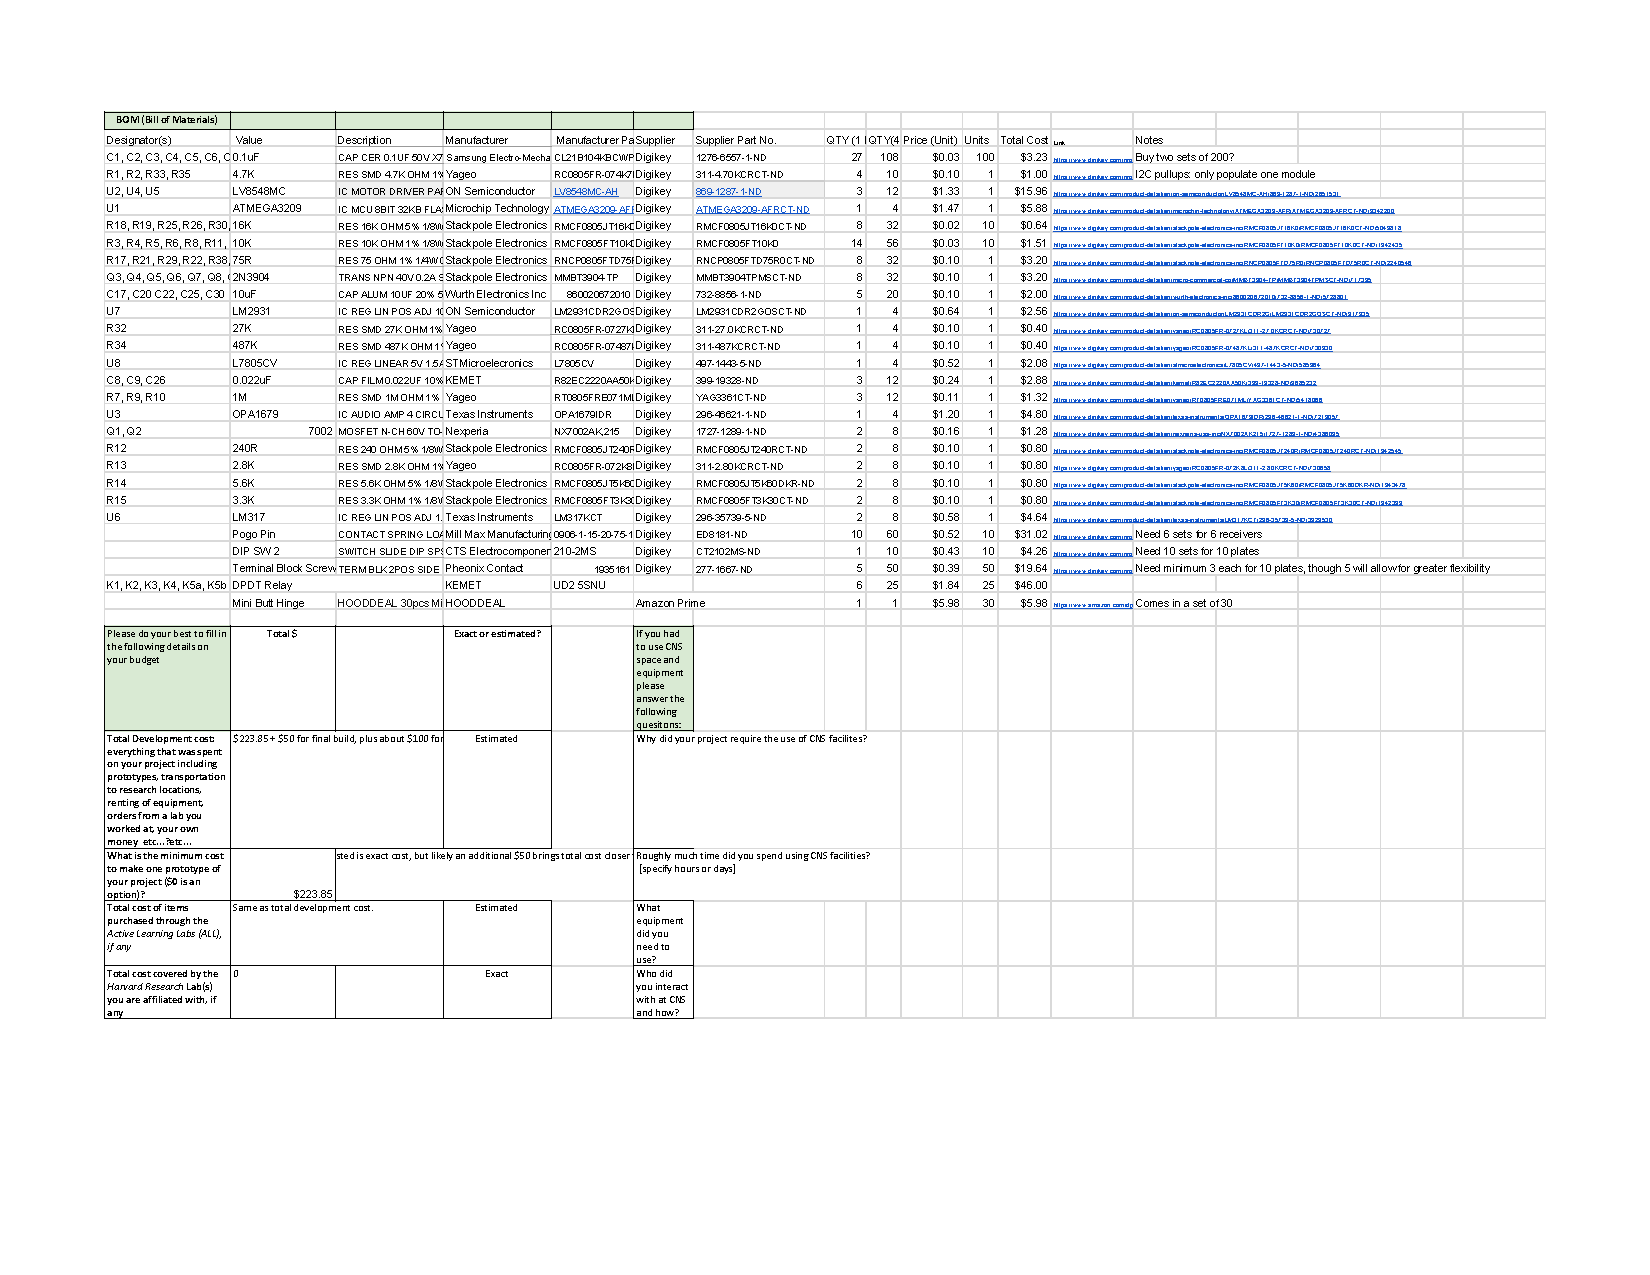
\includepdf[pages=-, angle=90, scale=0.9, pagecommand={}]{FinalBudget.pdf}

	\sect{Module Schematic and Layout}
	The design files developed in Altium are shown below.  A hierarchical design was used, with the first page showing the highest level.  In green are the lower level blocks, which are described in the following pages.  Last is the circuit board layout.
	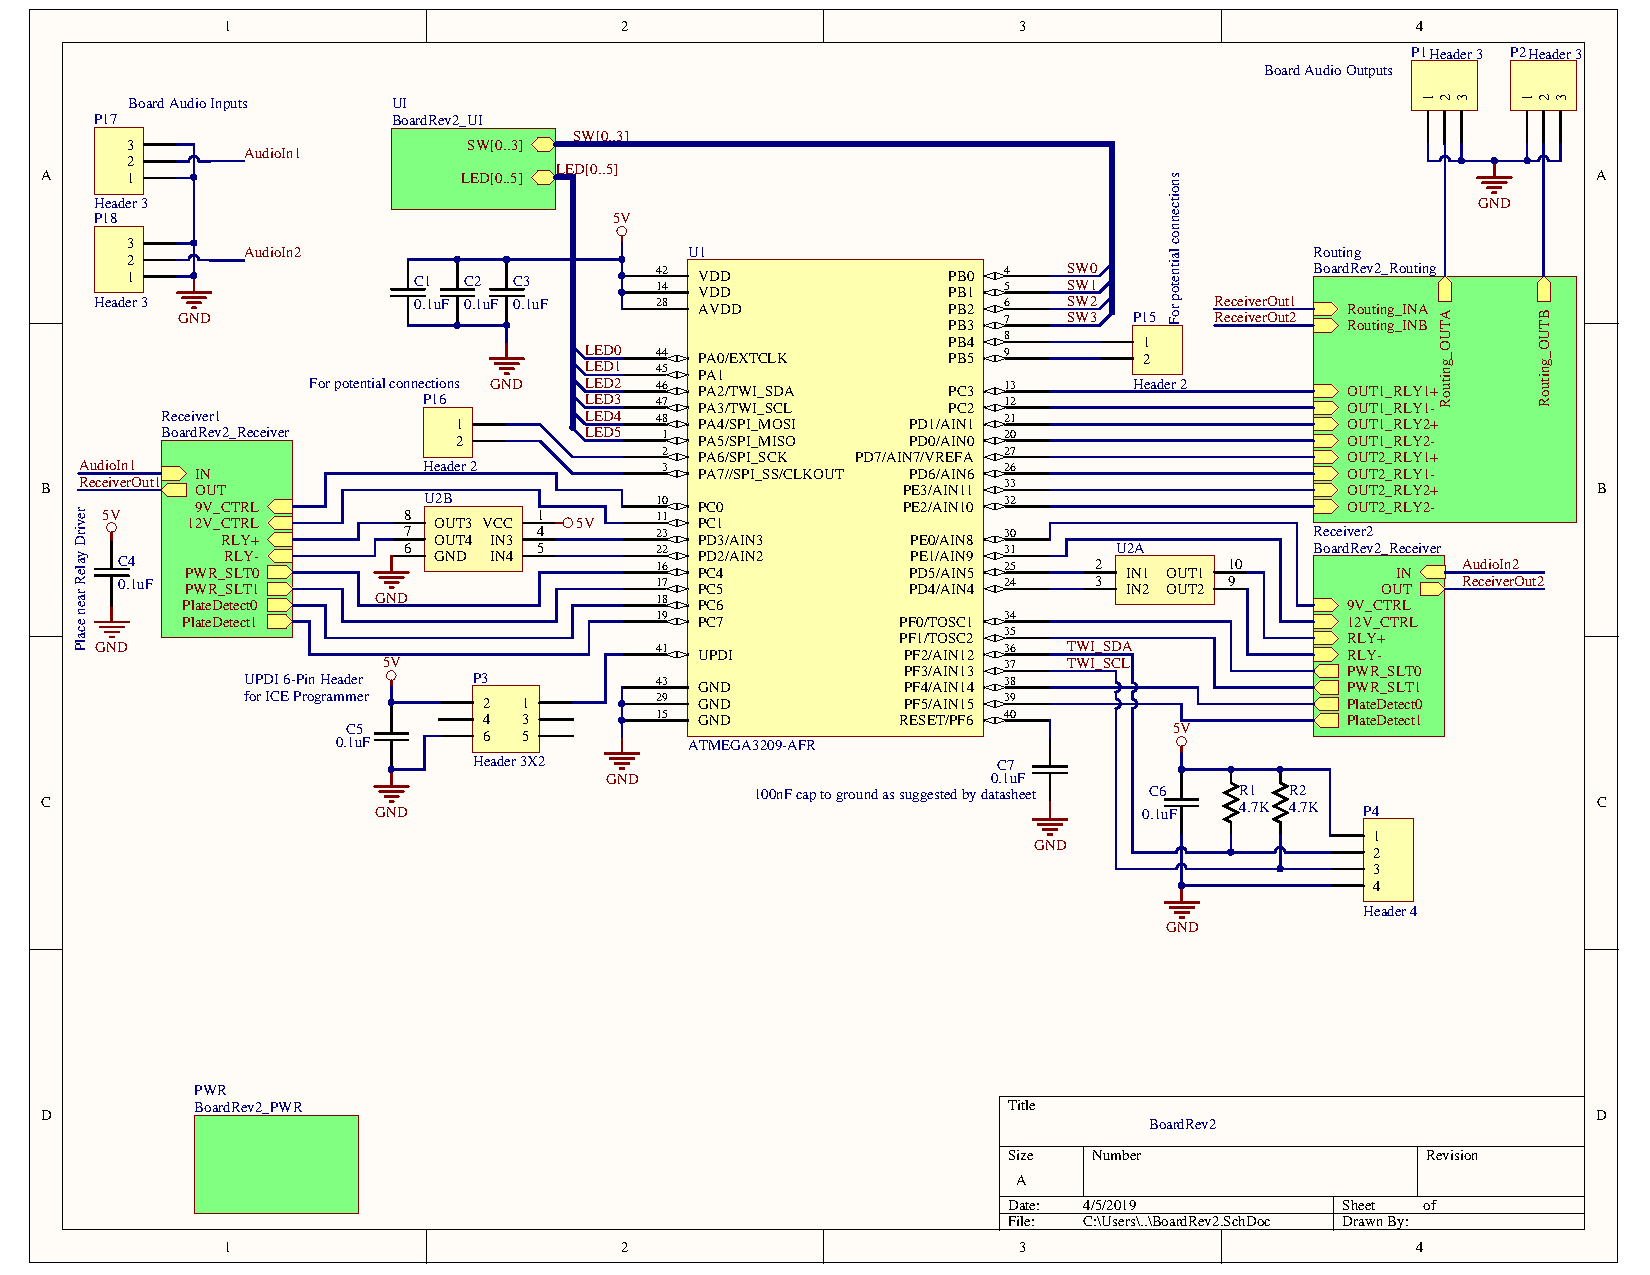
\includepdf[pages=1-6, angle=90, scale=0.8, pagecommand={}]{ReceiverBoardRev2.pdf}

	\sect{Global I/O Board Layout}
	This is the circuit board layout for the master I/O board for the device. The four identical components in the upper left are the audio jacks, and the choke is the large square footprint at the bottom.  This board was built using a milling machine, so it was designed as a single-sided board.
	\begin{center}
		\centering
		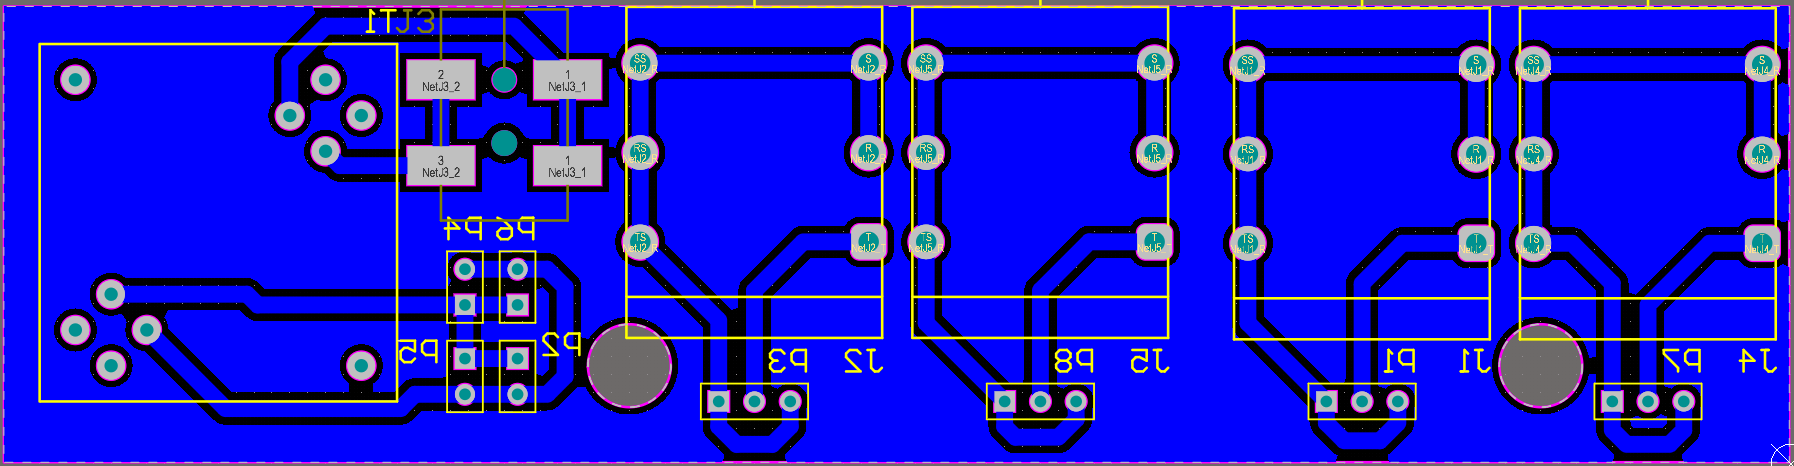
\includegraphics[width = \textwidth, angle=90]{FinalImages/IOBoardLayout}
	\end{center}
	\newpage

	\sect{SMD LED Fixtures for UI}
	This is the design for the fixtures to hold the SMD LEDs for the user interface.  In purple is the outline, which allowed 6 fixtures to be cut out at once and snapped apart.
	\begin{center}
		\centering
		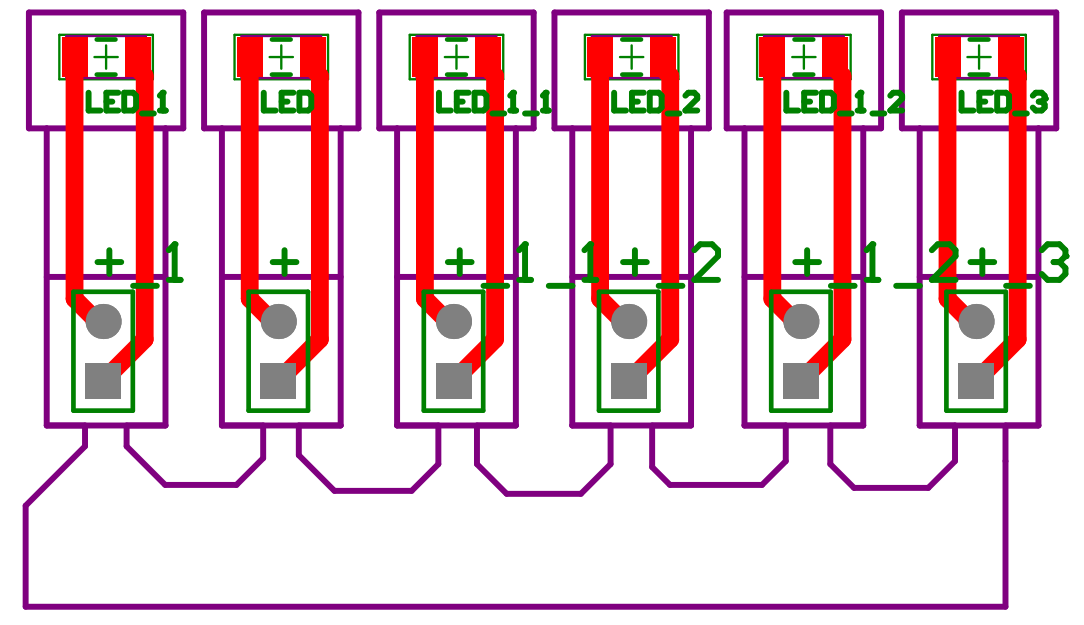
\includegraphics[width = \textwidth, angle=90]{FinalImages/SMDLEDfixture}
	\end{center}

\end{document}